\chapter[Models]{Physical and numerical models}

\section{Physical and mathematical description} 

Characteristic of compositional multiphase models is that the phases
are not only matter of a single chemical substance. Instead, their
composition in general includes several species, and for the mass transfer, 
the component behavior is quite different from the phase behavior. In the following, we
give some basic definitions and assumptions that are required for the
formulation of the model concept below. As an example, we take a
three-phase three-component system water-NAPL-gas
\cite{A3:class:2002a}. The modification for other multicomponent
systems is straightforward and can be found, e.\ g., in
\cite{A3:bielinski:2006,A3:acosta:2006}.

\subsection{Basic Definitions and Assumptions for the Compositional
  Model Concept}
\textbf{Components:}
The term {\it component} stands for constituents of the phases which
can be associated with a unique chemical species, or, more generally, with 
a group of species exploiting similar physical behavior. In this work, we
assume a water-gas-NAPL system composed of the phases water (subscript
$\text{w}$), gas ($\text{g}$), and NAPL ($\text{n}$). These phases are
composed of the components water (superscript $\text{w}$), air
($\text{a}$), and the organic contaminant ($\text{c}$) (see Fig.\
\ref{A3:fig:mundwtrans}).
%
\begin{figure}[hbt]
  \centering
  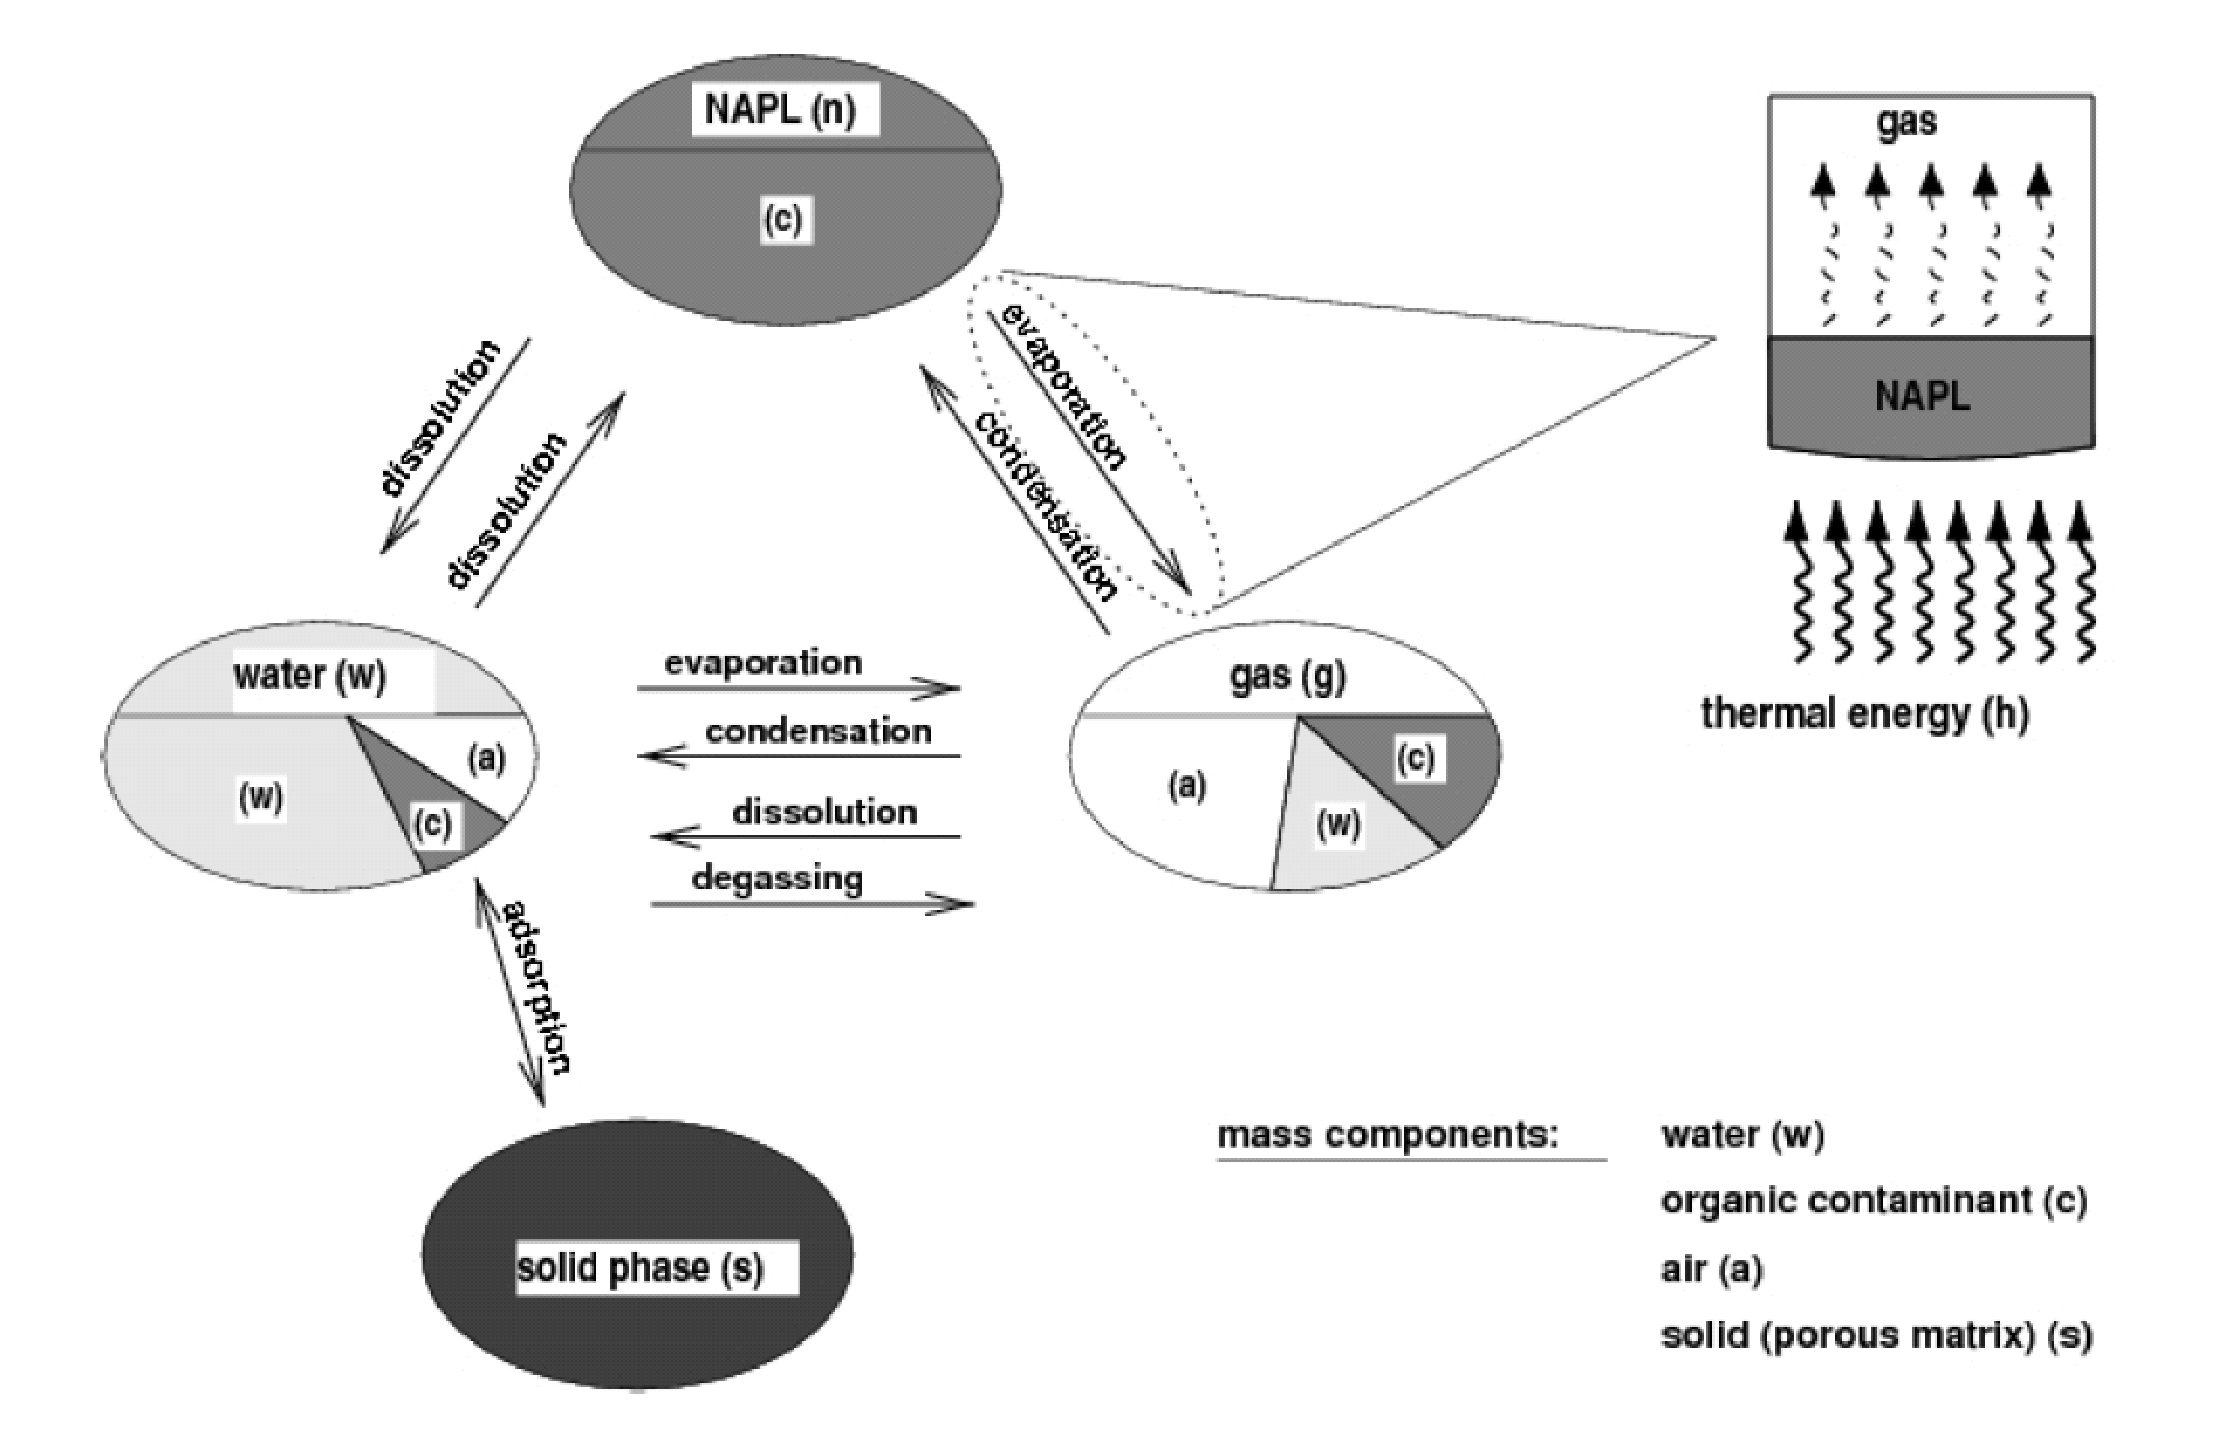
\includegraphics[width=0.7\linewidth]{EPS/masstransfer}
  \caption{Mass and energy transfer between the phases}
  \label{A3:fig:mundwtrans}
\end{figure}

\textbf{Equilibrium:}
For the nonisothermal multiphase processes in porous media under
consideration, we state that the assumption of local thermal
equilibrium is valid since flow velocities are small. We neglect
chemical reactions and biological decomposition and assume chemical
equilibrium.  Mechanical equilibrium is not valid in a porous medium, 
since discontinuities in pressure can occur across a fluid-fluid
interface due to capillary effects.

\textbf{Notation:} The index $\alpha \in \{\text{w}, \text{n}, \text{g}\}$ refers 
to the phase, while the superscript $\kappa \in \{\text{w}, \text{a}, \text{c}\}$ refers 
to the component. \\
\begin{tabular}{llll}
$p_\alpha$ & phase pressure & $\phi$ & porosity \\
$T$ & temperature & $K$ & absolute permeability tensor \\
$S_\alpha$ & phase saturation & $\tau$ & tortuosity \\
$x_\alpha^\kappa$ & mole fraction of component $\kappa$ in phase $\alpha$ & $\boldsymbol{g}$ & gravitational acceleration \\
$X_\alpha^\kappa$ & mass fraction of component $\kappa$ in phase $\alpha$ & $q^\kappa_\alpha$ & volume source term of $\kappa$ in $\alpha$ \\
$\varrho_{\text{mol},\alpha}$ & molar density of phase $\alpha$ & $u_\alpha$ & specific internal energy \\
$\varrho_{\alpha}$ & mass density of phase $\alpha$ & $h_\alpha$ & specific enthalpy \\
$k_{\text{r}\alpha}$ & relative permeability & $c_\text{s}$ & specific heat enthalpy \\
$\mu_\alpha$ & phase viscosity & $\lambda_\text{pm}$ & heat conductivity \\
$D_\alpha^\kappa$ & diffusivity of component $\kappa$ in phase $\alpha$ & $q^h$ & heat source term \\
$v_\alpha$ & Darcy velocity & $v_{a,\alpha}$  & advective velocity
\end{tabular}


\subsection{Balance Equations}
For the balance equations for multicomponent systems, it is in many
cases convenient to use a molar formulation of the continuity
equation. Considering the mass conservation for each component allows
us to drop source/sink terms for describing the mass transfer between
phases. Then, the
molar mass balance can be written as:
%
\begin{eqnarray}
  \label{A3:eqmass1}
  && \phi \frac{\partial (\sum_\alpha \varrho_{\text{mol}, \alpha}
    x_\alpha^\kappa S_\alpha )}{\partial t} \nonumber 
 - \sum\limits_\alpha \Div \left( \frac{k_{\text{r}
        \alpha}}{\mu_\alpha} \varrho_{\text{mol}, \alpha}
    x_\alpha^\kappa K (\grad p_\alpha -
    \varrho_{\alpha} \boldsymbol{g}) \right) \nonumber \\
  %
  \nonumber \\
  %
  && - \sum\limits_\alpha \Div \left( \tau \phi S_\alpha D_\alpha^\kappa \varrho_{\text{mol},
      \alpha} \grad x_\alpha^\kappa \right) \nonumber 
 - q^\kappa = 0, \qquad \kappa \in \{\text{w,a,c}\}.
\end{eqnarray}

The component mass balance can also be written in terms of mass fractions 
by replacing molar densities by mass densities and mole by mass fractions.
To obtain a single conserved quantity in the temporal derivative, the total 
concentration, representing the mass of one component per unit volume, is defined as
\begin{displaymath}
C^\kappa = \sum_\alpha \phi S_\alpha \varrho_{\text{mass},\alpha} X_\alpha^\kappa \; .
\end{displaymath}
Using this definition, the component mass balance is written as:

\begin{eqnarray}
  \label{A3:eqmass2}
  &&  \frac{\partial C^\kappa}{\partial t} = 
  \sum\limits_\alpha \Div \left( \frac{k_{\text{r}
        \alpha}}{\mu_\alpha} \varrho_{\text{mass}, \alpha}
    X_\alpha^\kappa K (\grad p_\alpha +
    \varrho_{\text{mass}, \alpha} \boldsymbol{g}) \right) \nonumber \\
  %
  \nonumber \\
  %
  && + \sum\limits_\alpha \Div \left( \tau \phi S_\alpha D_\alpha^\kappa \varrho_{\text{mass},
      \alpha} \grad X_\alpha^\kappa \right) \nonumber 
 + q^\kappa = 0, \qquad \kappa \in \{\text{w,a,c}\}.
\end{eqnarray}


In the case of non-isothermal systems, we further have to balance the
thermal energy. We assume fully reversible processes, such that entropy
is not needed as a model parameter. Furthermore, we neglect 
dissipative effects and the heat transport due to molecular
diffusion. The heat balance can then be
formulated as:
%
\begin{eqnarray}
  \label{A3:eqenergmak1}
  && \phi \frac{\partial \left( \sum_\alpha \varrho_{\alpha}
      u_\alpha S_\alpha \right)}{\partial t} + \left( 1 -
    \phi \right) \frac{\partial \varrho_{\text{s}} c_{\text{s}}
    T}{\partial t} \nonumber 
 - \Div \left( \lambda_{\text{pm}} \grad T \right)
  \nonumber \\
  %
  \nonumber \\
  %
  && - \sum\limits_\alpha \Div \left( \frac{k_{\text{r}
        \alpha}}{\mu_\alpha} \varrho_{\alpha} h_\alpha
    K \left( \grad p_\alpha - \varrho_{\alpha}
      \boldsymbol{g} \right) \right) \nonumber 
 - q^h \; = \; 0.
\end{eqnarray}

In order to close the system, supplementary constraints for capillary pressure, saturations and mole
fractions are needed, \cite{A3:helmig:1997}. 
According to the Gibbsian phase rule, the number of degrees of freedom
in a non-isothermal compositional multiphase system is equal to the
number of components plus one. This means we need as many independent
unknowns in the system description. The
available primary variables are, e.\ g., saturations, mole/mass
fractions, temperature, pressures, etc.




\section{Available models} 
The following description of the available models is automatically extracted 
from the Doxygen documentation. \textbf{TODO}: Unify notation. 

\subsection{Fully coupled models} 

\subsubsection{The single-phase model: OnePBoxModel} 
Single phase isothermal flow model is implemented for compressible flow. \begin{align*} \phi \frac{\partial \varrho}{\partial t} + \vec{\nabla} \cdot (- \varrho \frac{\bar{\bar{K}}}{\mu} ( \nabla p -\varrho \vec{g})) = q \end{align*} which is discretized by this model using vertex centered finite volume (box) scheme as spatial and the implicit Euler method as time discretization. However, the model can also be used for incompressible single pahse flow modeling, when in problem file a fluid with constant density is chosen. 


\subsubsection{The single-phase, two-component model:  OnePTwoCBoxModel} 



\subsubsection{The two-phase model using Richards' assumption: RichardsBoxModel} 
%%%%%%%%%%%%%%%%%%%%%%%%%%%%%%%%%%%%%%%%%%%%%%%%%%%%%%%%%%%%%%%%%
% This file has been autogenerated from the LaTeX part of the   %
% doxygen documentation; DO NOT EDIT IT! Change the model's .hh %
% file instead!!                                                %
%%%%%%%%%%%%%%%%%%%%%%%%%%%%%%%%%%%%%%%%%%%%%%%%%%%%%%%%%%%%%%%%%


This model implements a variant of the Richards equation for quasi-\/twophase flow. In the unsaturated zone, Richards' equation is frequently used to calculate the water distribution above the groundwater level. It can be derived from the twophase equations, i.e. \[ \frac{\partial\;\phi S_\alpha \rho_\alpha}{\partial t} - \mathbf{div} \left\{ \rho_\alpha \frac{k_{r\alpha}}{\mu_\alpha}\;K \mathbf{grad}\left[ p_\alpha - g\rho_\alpha \right] \right\} = q_\alpha, \] where $\alpha \in \{w, n\}$ is the fluid phase, $\rho_\alpha$ is the fluid density, $S_\alpha$ is the fluid saturation, $\phi$ is the porosity of the soil, $k_{r\alpha}$ is the relative permeability for the fluid, $\mu_\alpha$ is the fluid's dynamic viscosity, $K$ is the intrinsic permeability, $p_\alpha$ is the fluid pressure and $g$ is the potential of the gravity field.

In contrast to the full twophase model, the Richards model assumes gas as the non-\/wetting fluid and that it exhibits a much lower viscosity than the (liquid) wetting phase. (For example at atmospheric pressure and at room temperature, the viscosity of air is only about $1\%$ of the viscosity of liquid water.) As a consequence, the $\frac{k_{r\alpha}}{\mu_\alpha}$ term typically is much larger for the gas phase than for the wetting phase. For this reason, the Richards model assumes that $\frac{k_{rn}}{\mu_n}$ tends to infinity. This implies that the pressure of the gas phase is equivalent to a static pressure and can thus be specified externally and that therefore, mass conservation only needs to be considered for the wetting phase.

The model thus choses the absolute pressure of the wetting phase $p_w$ as its only primary variable. The wetting phase saturation is calculated using the inverse of the capillary pressure, i.e. \[ S_w = p_c^{-1}(p_n - p_w) \] holds, where $p_n$ is a given reference pressure. Nota bene that the last step is assumes that the capillary pressure-\/saturation curve can be inverted uniquely, so it is not possible to set the capillary pressure to zero when using the Richards model!



\subsubsection{The two-phase model: TwoPBoxModel}
You can pick the formulation by setting the \char`\"{}Formulation\char`\"{} property. The default is pW-Sn. 


\subsubsection{The non-isothermal two-phase model: TwoPNIBoxModel} 
%%%%%%%%%%%%%%%%%%%%%%%%%%%%%%%%%%%%%%%%%%%%%%%%%%%%%%%%%%%%%%%%%
% This file has been autogenerated from the LaTeX part of the   %
% doxygen documentation; DO NOT EDIT IT! Change the model's .hh %
% file instead!!                                                %
%%%%%%%%%%%%%%%%%%%%%%%%%%%%%%%%%%%%%%%%%%%%%%%%%%%%%%%%%%%%%%%%%


Adaption of the BOX scheme to the non-\/isothermal twophase flow model. This model implements a non-\/isothermal two-\/phase flow of two completely immiscible fluids $\alpha \in \{ w, n \}$. Using the standard multiphase Darcy approach, the mass conservation equations for both phases can be described as follows: \begin{eqnarray*} && \phi \frac{\partial (\varrho_\alpha S_\alpha )}{\partial t} - \text{div} \left\{ \varrho_\alpha \frac{k_{r\alpha}}{\mu_\alpha} \mbox{\bf K} (\text{grad}\, p_\alpha - \varrho_{\alpha} \mbox{\bf g}) \right\} - q_\alpha^\kappa = 0 \qquad \alpha \in \{w, n\} \end{eqnarray*} For the energy balance, local thermal equilibrium is assumed which results in one energy conservation equation for the porous solid matrix and the fluids: \begin{eqnarray*} && \phi \frac{\partial \left( \sum_\alpha \varrho_\alpha u_\alpha S_\alpha \right)}{\partial t} + \left( 1 - \phi \right) \frac{\partial (\varrho_s c_s T)}{\partial t} - \sum_\alpha \text{div} \left\{ \varrho_\alpha h_\alpha \frac{k_{r\alpha}}{\mu_\alpha} \mbox{\bf K} \left( \text{grad} \, p_\alpha - \varrho_\alpha \mbox{\bf g} \right) \right\} \\ &-& \text{div} \left( \lambda_{pm} \text{grad} \, T \right) - q^h = 0, \qquad \alpha \in \{w, n\}. \end{eqnarray*}

The equations are discretized using a fully-\/coupled vertex centered finite volume (box) scheme as spatial and the implicit Euler method as time discretization.

Currently the model supports choosing either $p_w$, $S_n$ and $T$ or $p_n$, $S_w$ and $T$ as primary variables. The formulation which ought to be used can be specified by setting the {\ttfamily Formulation} property to either {\ttfamily TwoPNIIndices::pWsN} or {\ttfamily TwoPIndices::pNsW}. By default, the model uses $p_w$, $S_n$ and $T$.



\subsubsection{The two-phase, two-component model: TwoPTwoCBoxModel} 
%%%%%%%%%%%%%%%%%%%%%%%%%%%%%%%%%%%%%%%%%%%%%%%%%%%%%%%%%%%%%%%%%
% This file has been autogenerated from the LaTeX part of the   %
% doxygen documentation; DO NOT EDIT IT! Change the model's .hh %
% file instead!!                                                %
%%%%%%%%%%%%%%%%%%%%%%%%%%%%%%%%%%%%%%%%%%%%%%%%%%%%%%%%%%%%%%%%%


Adaption of the BOX scheme to the two-\/phase two-\/component flow model. This model implements two-\/phase two-\/component flow of two compressible and partially miscible fluids $\alpha \in \{ w, n \}$ composed of the two components $\kappa \in \{ w, a \}$. The standard multiphase Darcy approach is used as the equation for the conservation of momentum: \[ v_\alpha = - \frac{k_{r\alpha}}{\mu_\alpha} \mbox{\bf K} \left(\text{grad}\, p_\alpha - \varrho_{\alpha} \mbox{\bf g} \right) \]

By inserting this into the equations for the conservation of the components, one gets one transport equation for each component \begin{eqnarray} && \phi \frac{\partial (\sum_\alpha \varrho_\alpha X_\alpha^\kappa S_\alpha )} {\partial t} - \sum_\alpha \text{div} \left\{ \varrho_\alpha X_\alpha^\kappa \frac{k_{r\alpha}}{\mu_\alpha} \mbox{\bf K} (\text{grad}\, p_\alpha - \varrho_{\alpha} \mbox{\bf g}) \right\} \nonumber \\ \nonumber \\ &-& \sum_\alpha \text{div} \left\{{\bf D_{\alpha, pm}^\kappa} \varrho_{\alpha} \text{grad}\, X^\kappa_{\alpha} \right\} - \sum_\alpha q_\alpha^\kappa = 0 \qquad \kappa \in \{w, a\} \, , \alpha \in \{w, g\} \end{eqnarray}

This is discretized using a fully-\/coupled vertex centered finite volume (box) scheme as spatial and the implicit Euler method as temporal discretization.

By using constitutive relations for the capillary pressure $p_c = p_n - p_w$ and relative permeability $k_{r\alpha}$ and taking advantage of the fact that $S_w + S_n = 1$ and $X^\kappa_w + X^\kappa_n = 1$, the number of unknowns can be reduced to two. The used primary variables are, like in the two-\/phase model, either $p_w$ and $S_n$ or $p_n$ and $S_w$. The formulation which ought to be used can be specified by setting the {\ttfamily Formulation} property to either TwoPTwoCIndices::pWsN or TwoPTwoCIndices::pNsW. By default, the model uses $p_w$ and $S_n$. Moreover, the second primary variable depends on the phase state, since a primary variable switch is included. The phase state is stored for all nodes of the system. Following cases can be distinguished:
\begin{itemize}
\item Both phases are present: The saturation is used (either $S_n$ or $S_w$, dependent on the chosen {\ttfamily Formulation}), as long as $ 0 < S_\alpha < 1$.
\item Only wetting phase is present: The mass fraction of, e.g., air in the wetting phase $X^a_w$ is used, as long as the maximum mass fraction is not exceeded ( $X^a_w<X^a_{w,max}$)
\item Only non-\/wetting phase is present: The mass fraction of, e.g., water in the non-\/wetting phase, $X^w_n$, is used, as long as the maximum mass fraction is not exceeded ( $X^w_n<X^w_{n,max}$)
\end{itemize}



\subsubsection{The non-isothermal two-phase, two-component model: TwoPTwoCNIBoxModel} 
This implements a non-isothermal two-phase two-component model with Pw and Sn/X as primary unknowns. You can use Pn and Sw/X as primary variables if you set the Formulation property to pNsW. 



\subsection{Decoupled models}

\subsubsection{FractionalFlow Model}
\input{ModelDescriptions/2pdecoupledmodel}

\subsubsection{Decoupled2p2c}

(Extracted from decoupled2p2c.hh:) 
This implementation is written for a liquid-gas system. For the physical description of gas and liquid derivations of the classes \doxyref{Gas\_\-GL}{p.}{classDune_1_1Gas__GL} and \doxyref{Liquid\_\-GL}{p.}{classDune_1_1Liquid__GL} have to be provided. The template parameters are the used grid class and the desired number type (usually double) The pressure equation is given as $ -\frac{\partial V}{\partial p}\frac{\partial p}{\partial t}+\sum_{\kappa}\frac{\partial V}{\partial m^{\kappa}}\nabla\cdot\left(\sum_{\alpha}C_{\alpha}^{\kappa}\mathbf{v}_{\alpha}\right)=\sum_{\kappa}\frac{\partial V}{\partial m^{\kappa}}q^{\kappa}$ See paper SPE 99619 for derivation. The transport equation is $ \frac{\partial C^\kappa}{\partial t} = - \nabla \cdot \sum{C_\alpha^\kappa f_\alpha {\bf v}} + q^\kappa $ 






%%% Local Variables: 
%%% mode: latex
%%% TeX-master: "dumux-handbook"
%%% End: 
